%% Use the hmcposter class with the thesis document-class option.
\documentclass[thesis]{hmcposter}
\usepackage{graphicx}
\usepackage{natbib}
\usepackage{booktabs}
\usepackage{subfig}
\usepackage{amsmath}
\usepackage{textcomp}
\usepackage{url}

%% Author of the thesis.
\author{Claire Connelly}

%% The year of your thesis poster's creation.
\posteryear{2008}

%% Thesis Title.
\title{Putting Together a Poster for Presentation Days}

%% The name of the class for which the poster was created.
%% Generally we see posters for thesis and Clinic, but sometimes
%% other classes require or allow the creation of posters to
%% communicate the results of a project.
%% 
%% Use the format Math nnn: Class Title.
\class{Math 197: Senior Thesis}

%% Advisor(s) name or names.  Separate with \and.
\advisor{Melissa O'Neill \and Lesley Ward}

%% Reader(s) name or names.  Separate with \and.
\reader{Melissa O'Neill \and Charlie Watts}

%% Optional -- if you are especially concerned about intellectual
%% property issues (maybe you have some potentially patentable
%% material in your thesis), you can use the \copyrightholder
%% command to supply a name for a copyright holder for your
%% poster.  Note that under U.S. law, all works are under
%% copyright from the moment of creation; the copyright statement
%% is merely making your claim obvious.
%%
%% This command is also useful if you are sharing copyright of the
%% poster with someone else (e.g., a student collaborator, your
%% advisor, an organization).
%%
\copyrightholder{Claire~M. Connelly and the Department of
  Mathematics, Harvey Mudd College}


%% Define the \BibTeX command, used in our example document.
\providecommand{\bibtex}{{\rmfamily B\kern-.05em%
    \textsc{i\kern-.025em b}\kern-.08em%
    T\kern-.1667em\lower.7ex\hbox{E}\kern-.125emX}}


\pagestyle{fancy}

\begin{document}

\begin{poster}

\section{Introduction}
% Note that we're not labeling sections because you shouldn't be
% doing a lot of referring back and forth in your poster---let the
% interested folks read your thesis or Clinic report, or ask
% questions.

Describe the basics about your thesis or project here---briefly!  An
image such as Figure~\ref{fig:our-poster} can help jazz up the
introduction and get people interested in your poster.

\begin{figure}
\begin{center}
\fbox{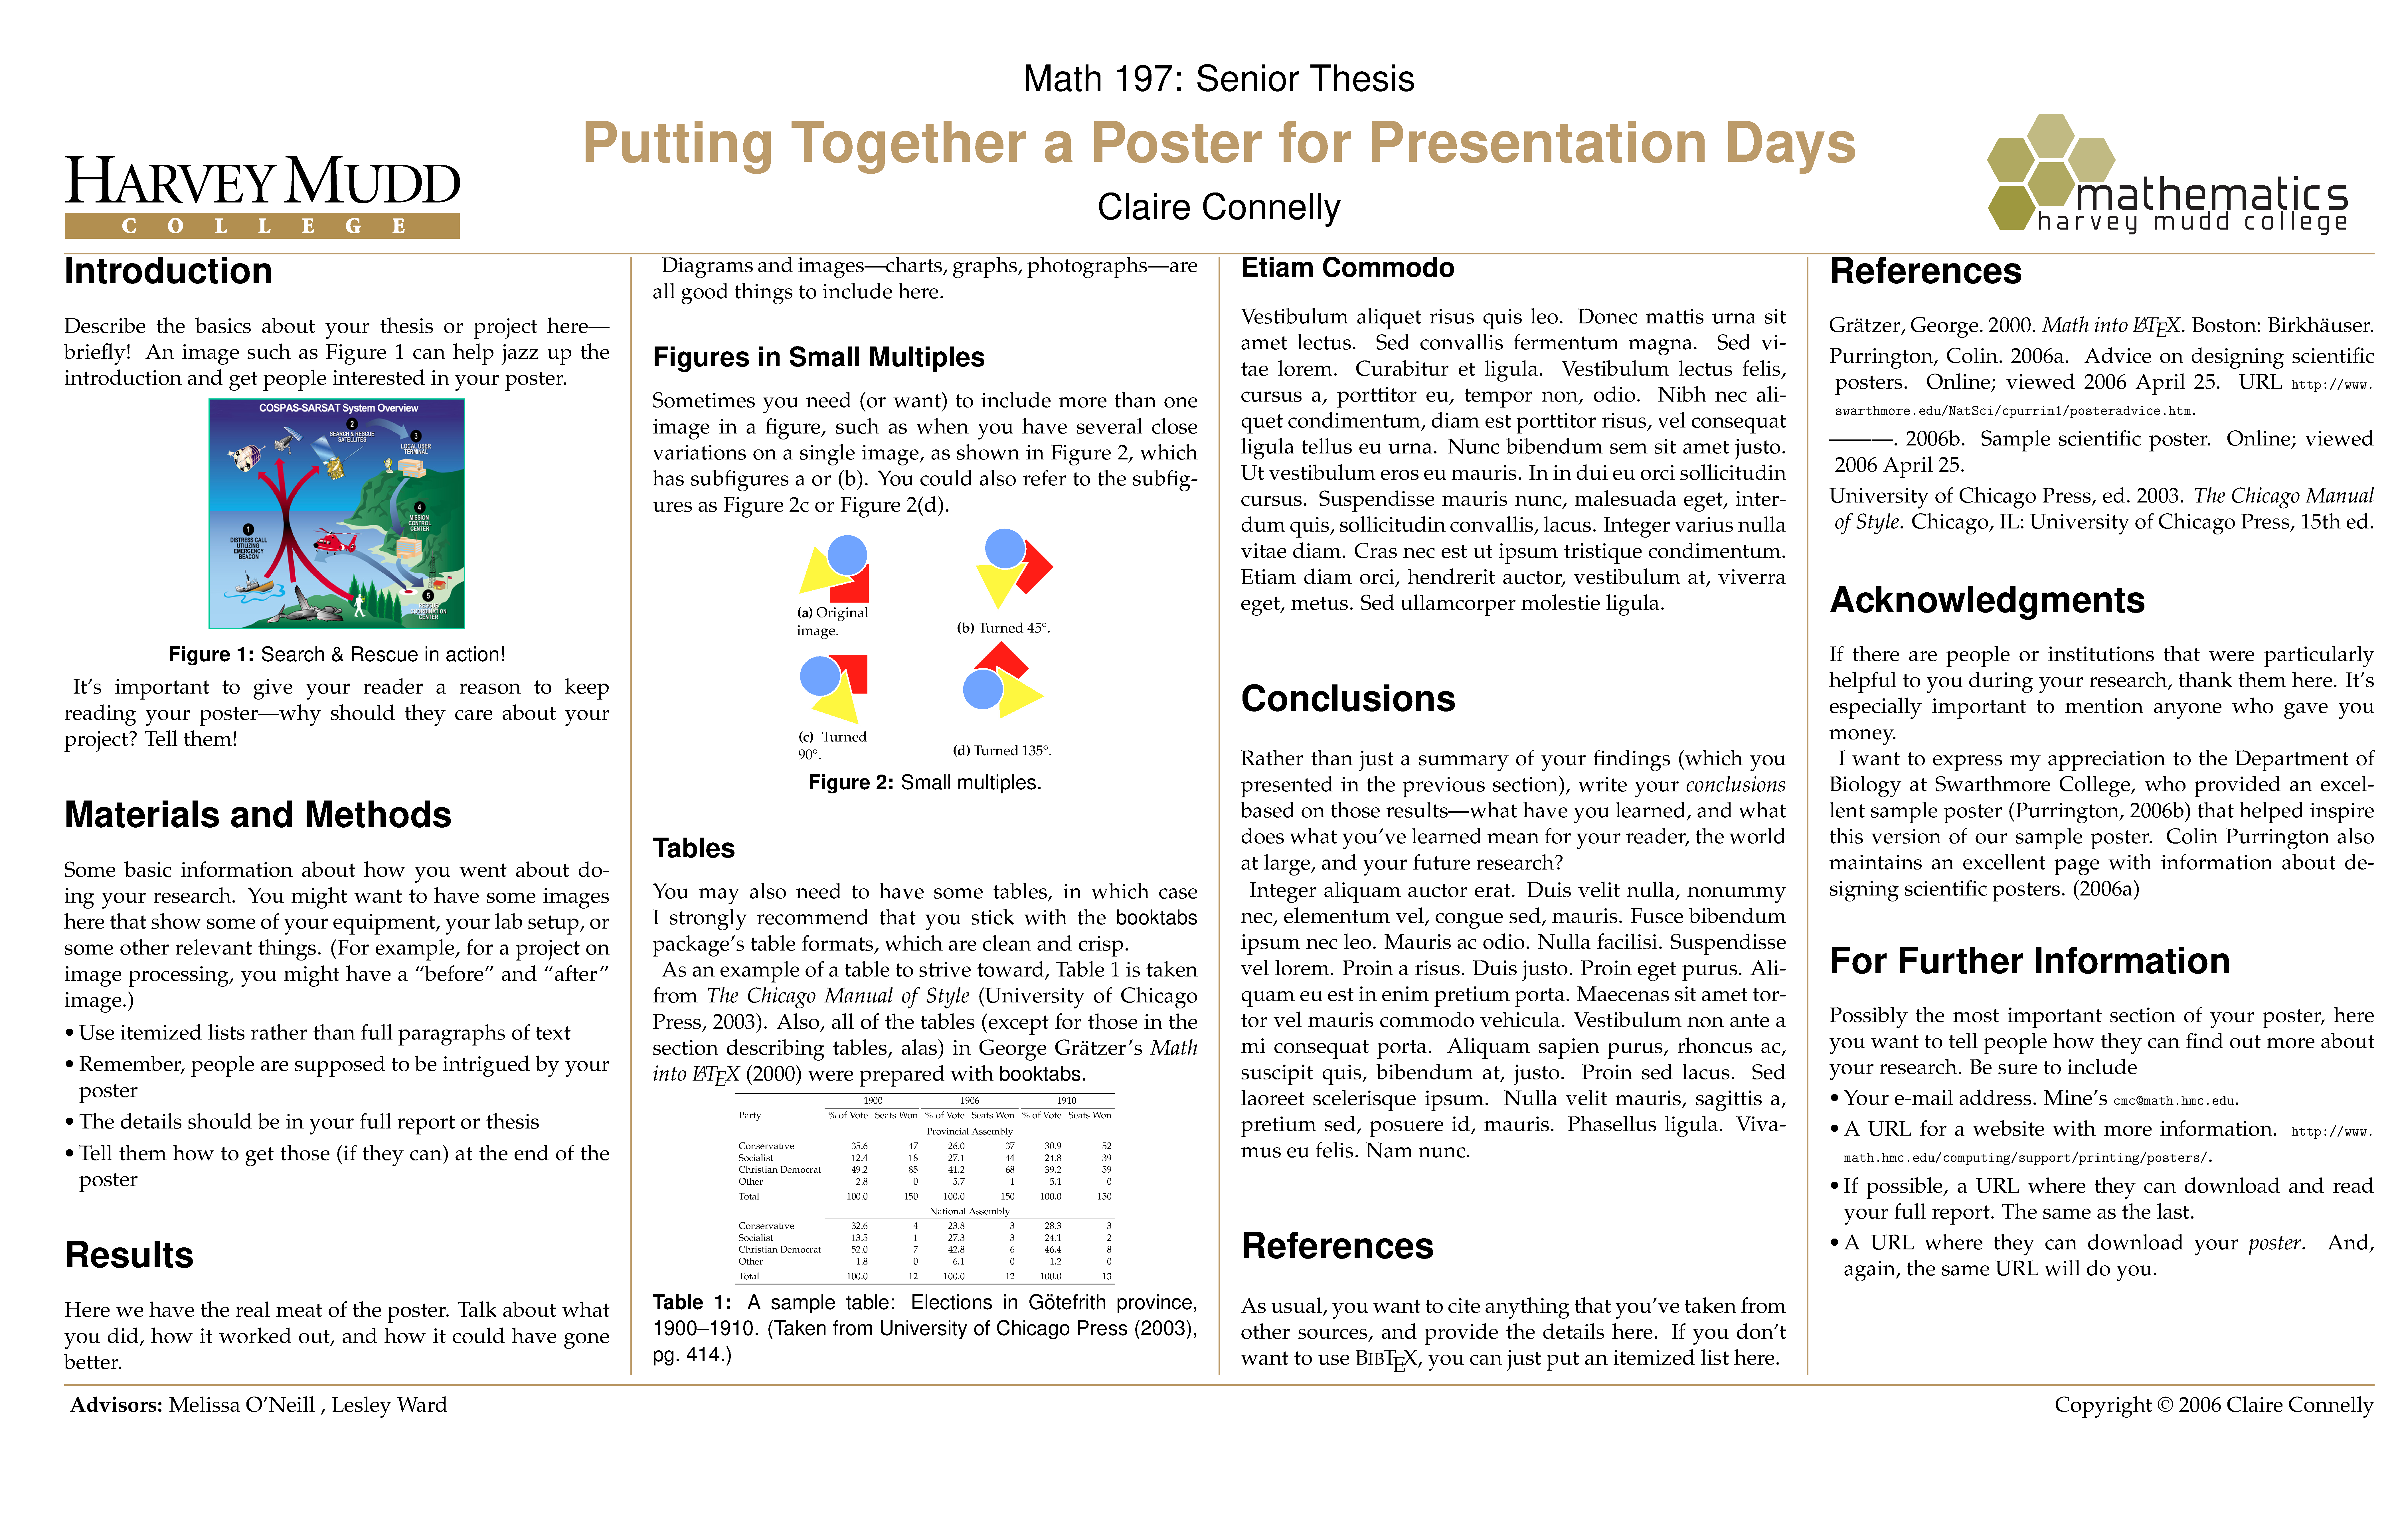
\includegraphics[width=6in]{sampleposter}}
\caption{What a great poster!}%
\label{fig:our-poster}
\end{center}
\end{figure}

It's important to give your reader a reason to keep reading your
poster---why should they care about your project?  Tell them!


\section{Materials and Methods}%

Some basic information about how you went about doing your
research.  You might want to have some images here that show some of
your equipment, your lab setup, or some other relevant things.  (For
example, for a project on image processing, you might have a
``before'' and ``after'' image.)

\begin{itemize}
\item Use itemized lists rather than full paragraphs of text
\item Remember, people are supposed to be intrigued by your poster
\item The details should be in your full report or thesis
\item Tell them how to get those (if they can) at the end of the poster
\end{itemize}


\section{Results}%

Here we have the real meat of the poster.  Talk about what you did,
how it worked out, and how it could have gone better.

Diagrams and images---charts, graphs, photographs---are all good
things to include here.


\subsection{Figures in Small Multiples}

Sometimes you need (or want) to include more than one image in a
figure, such as when you have several close variations on a single
image, as shown in Figure~\ref{fig:small-multiples}, which has
subfigures \subref*{fig:small-mults-orig} or
\subref{fig:small-mults-45}.  You could also refer to the subfigures
as Figure~\ref{fig:small-mults-90} or
Figure~\ref{fig:small-multiples}\subref{fig:small-mults-135}.

\begin{figure}
  \centering
        \subfloat[][Original image.]{\scalebox{.75}{
\includegraphics{shapes}}%
                \label{fig:small-mults-orig}%
        }\qquad\qquad
        \subfloat[][Turned 45\textdegree.]{
\includegraphics[scale=.75,origin=c,angle=45]{shapes}%
                \label{fig:small-mults-45}%
        }\\
        \subfloat[][Turned 90\textdegree.]{\scalebox{.75}{
\includegraphics[origin=c,angle=90]{shapes}}%
                \label{fig:small-mults-90}%
        }\qquad\qquad
        \subfloat[][Turned 135\textdegree.]{\scalebox{.75}{
\includegraphics[origin=c,angle=135]{shapes}}%
                \label{fig:small-mults-135}%
        }
  \caption[Small multiples]{Small multiples.}%
  \label{fig:small-multiples}
\end{figure}

\subsection{Tables}

You may also need to have some tables, in which case I strongly
recommend that you stick with the \textsf{booktabs} package's table
formats, which are clean and crisp. \citep{fear-booktab}

As an example of a table to strive toward,
Table~\ref{tab:chicago-table} is taken from \emph{The Chicago Manual
  of Style} \citep{chicago}.  Also, all of the tables (except for
those in the section describing tables, alas) in George
Gr\"{a}tzer's \emph{Math into \LaTeX} \citeyearpar{gratzer-mil} were
prepared with \textsf{booktabs}.

\begin{table}
\begin{center}
%{\hspace{-1in}
%\begin{minipage}{\textwidth}

%% To make this complex table fit, we've had to shrink the text
%% down to the point that it is way too small for anyone to read.
%%
%% Don't do that in your poster -- either simplify any tables so
%% that they can be typeset full-size or drop them altogether and
%% just include them in your handout or in materials available on
%% your website.
\fontsize{22}{26.4}\selectfont
\begin{tabular}[c]{lrrrrrr}
\toprule
              & \multicolumn{2}{c}{1900} & \multicolumn{2}{c}{1906} & \multicolumn{2}{c}{1910}\\
\cmidrule(r){2-3}\cmidrule{4-5}\cmidrule(l){6-7}
Party         & \% of Vote  & Seats Won  & \% of Vote  & Seats Won  & \% of Vote  & Seats Won \\
\midrule
\addlinespace
              & \multicolumn{6}{c}{Provincial Assembly}\\
\cmidrule{2-7}
Conservative  & 35.6        &  47        & 26.0        & 37         & 30.9        & 52\\
Socialist     & 12.4        &  18        & 27.1        & 44         & 24.8        & 39\\
Christian Democrat & 49.2   &  85        & 41.2        & 68         & 39.2        & 59\\
Other         & 2.8         &  0         & 5.7         & 1          & 5.1         & 0\\
\addlinespace
Total& 100.0       &  150       & 100.0       & 150        & 100.0       & 150\\
\addlinespace
              & \multicolumn{6}{c}{National Assembly}\\
\cmidrule{2-7}
Conservative  & 32.6        &   4        & 23.8        &  3         & 28.3        & 3\\
Socialist     & 13.5        &   1        & 27.3        &  3         & 24.1        & 2\\
Christian Democrat & 52.0   &   7        & 42.8        &  6         & 46.4        & 8\\
Other         & 1.8         &   0        & 6.1         &  0         & 1.2         & 0\\
\addlinespace
Total& 100.0       &  12        & 100.0       & 12         & 100.0       & 13\\
\bottomrule
\end{tabular}
%\end{minipage}
%}
\caption[A sample table: Elections in G\"{o}tefrith province,
1900--1910]{A sample table: Elections in
  G\"{o}tefrith province, 1900--1910.  (Taken from \cite{chicago},
  pg.~414.)}%
\label{tab:chicago-table}
\end{center}
\end{table}


\subsection{Etiam Commodo}%
\label{sec:etiam-commodo}

Vestibulum aliquet risus quis leo. Donec mattis urna sit amet
lectus. Sed convallis fermentum magna. Sed vitae lorem. Curabitur et
ligula. Vestibulum lectus felis, cursus a, porttitor eu, tempor non,
odio. Nibh nec aliquet condimentum, diam est porttitor risus, vel
consequat ligula tellus eu urna. Nunc bibendum sem sit amet
justo. Ut vestibulum eros eu mauris. In in dui eu orci sollicitudin
cursus. Suspendisse mauris nunc, malesuada eget, interdum quis,
sollicitudin convallis, lacus. Integer varius nulla vitae diam. Cras
nec est ut ipsum tristique condimentum. Etiam diam orci, hendrerit
auctor, vestibulum at, viverra eget, metus. Sed ullamcorper molestie
ligula.


\section{Conclusions}

Rather than just a summary of your findings (which you presented in
the previous section), write your \emph{conclusions} based on those
results---what have you learned, and what does what you've learned
mean for your reader, the world at large, and your future research?

Integer aliquam auctor erat. Duis velit nulla, nonummy nec,
elementum vel, congue sed, mauris. Fusce bibendum ipsum nec
leo. Mauris ac odio. Nulla facilisi. Suspendisse vel lorem. Proin a
risus. Duis justo. Proin eget purus. Aliquam eu est in enim pretium
porta. Maecenas sit amet tortor vel mauris commodo
vehicula. Vestibulum non ante a mi consequat porta. Aliquam sapien
purus, rhoncus ac, suscipit quis, bibendum at, justo. Proin sed
lacus. Sed laoreet scelerisque ipsum. Nulla velit mauris, sagittis
a, pretium sed, posuere id, mauris. Phasellus ligula. Vivamus eu
felis. Nam nunc.




\section{Formatting References}

As usual, you want to cite anything that you've taken from other
sources, and provide the details here.  If you don't want to use
\bibtex, you can just put an itemized list here instead.

% Force a column break here so the references begin the next column.
\columnbreak

%% References.
%% Note that BibTeX will add its own section-level header, ``References''.

\bibliographystyle{hmcmath}
\bibliography{sampleposter}


\section{Acknowledgments}

If there are people or institutions that were particularly helpful
to you during your research, thank them here.  It's especially
important to mention anyone who gave you money.

I want to express my appreciation to the Department of Biology at
Swarthmore College, who provided an excellent sample poster
\citep{swarthmore-poster} that helped inspire this version of our
sample poster.  Colin Purrington also maintains an excellent page
with information about designing scientific
posters. \citeyearpar{purrington-sciposters}


\section{For Further Information}

Possibly the most important section of your poster!  Tell people
how they can find out more about your research.  Be sure to
include
\begin{itemize}
\item Your e-mail address.  Mine's \url{cmc@math.hmc.edu}.
\item A URL for a website with more information.  \url{http://www.math.hmc.edu/computing/support/printing/posters/}.
\item If possible, a URL where they can download and read your full
  report.  The same as the last.
\item A URL where they can download your \emph{poster}.  And, again,
  the same URL will do you.
\end{itemize}



\end{poster}

\end{document}

 
